%! Author = Juniell
%! Date = 31.05.2021

% Preamble
\documentclass[a4paper, 14pt]{extarticle}

% Packages
\usepackage[T2A]{fontenc}
\usepackage{natbib}
\usepackage{graphicx}
\usepackage[english, russian]{babel}
\usepackage{fontspec}
\usepackage{amsmath}
\usepackage{amsfonts}
\usepackage{amssymb}
\usepackage{amsthm}
\usepackage{mathtools}
\usepackage{mathrsfs}
\usepackage{fullpage}
\usepackage{ulem}
\usepackage{setspace}
\usepackage{listings}
\usepackage{indentfirst}
\usepackage[left=2cm,right=1.5cm,top=2cm,bottom=2cm]{geometry}
\usepackage{xcolor}
\usepackage{float}
\usepackage{csquotes}
\usepackage{hyperref}
\usepackage{graphics}

\definecolor{urlcolor}{HTML}{0000FF} % цвет ссылок
\definecolor{linkcolor}{HTML}{000000} % цвет гиперссылок
\hypersetup{pdfstartview=FitH, linkcolor=linkcolor, urlcolor=urlcolor, colorlinks=true}

\setmainfont{Times New Roman}
\setlength{\parindent}{5ex}
\setlength{\parskip}{1em}
\renewcommand{\baselinestretch}{1}

\graphicspath{{resources/Images}}

\definecolor{buzzlightyear}{HTML}{8757A5}
\definecolor{grass}{HTML}{738D06}
\definecolor{literal}{HTML}{F18A2B}
\definecolor{commentcolor}{HTML}{8E908B}

\lstdefinestyle{habrstyle}{
    backgroundcolor=\color{white},
    commentstyle=\color{commentcolor},
    keywordstyle=\bfseries\color{buzzlightyear},
    numberstyle=\tiny\color{commentcolor},
    stringstyle=\color{grass},
    basicstyle=\ttfamily\footnotesize,
    breakatwhitespace=false,
    breaklines=true,
    captionpos=b,
    keepspaces=true,
    numbers=left,
    numbersep=5pt,
    showspaces=false,
    showstringspaces=false,
    showtabs=false,
    tabsize=4,
    language=Python
}

\lstset{style=habrstyle}

% Document
\begin{document}
% Титульный лист
    \begin{center}
        \begin{center}
            \hfill \break
            \normalsize{Санкт-Петербургский государственный политехнический}\\
            \normalsize{университет Петра Великого}\\
            \hfill \break
            \normalsize{\textbf{Высшая школа интеллектуальных систем и}}\\
            \normalsize{\textbf{суперкомпьютерных технологий}}\\
            \hfill \break
            \hfill \break
            \hfill \break
            \hfill \break
            \hfill \break
            \normalsize{Отчёт по лабораторной работе №10}\\
            \normalsize{Дисциплина: Телекоммуникационные технологии}\\
            \normalsize{Тема: Линейные стационарные системы}\\
        \end{center}
        \hfill \break
        \hfill \break
        \hfill \break
        \hfill \break
        \hfill \break
        \hfill \break
        \hfill \break
        \hfill \break
        \hfill \break
        \hfill \break
        \begin{tabbing}
            Выполнил студент гр. 3530901/80201 \`В.А. Пучкина\\
            \\
            Преподаватель: \`Н.В. Богач\\
        \end{tabbing}
        \hfill \break
        \hfill \break
        \hfill \break
        \hfill \break
        \begin{center}
            Санкт-Петербург\\
            2021
        \end{center}
        \thispagestyle{empty}
    \end{center}

% Оглавление
    \newpage
    \tableofcontents

% Список иллюстраций
    \newpage
    \listoffigures

% Список листингов
    \newpage
    \lstlistoflistings

% ---------------------------------------------- Упражнение 10.1 ----------------------------------------------
    \newpage
    \section{Упражнение 10.1}
    \label{sec:task1}

    В разделе "Акустическая характеристика" умножение ДПФ сигнала на передаточную функцию соответствует
    круговой свёртке, но в предположении периодичности сигнала. В результате которой можно заметить,
    что на выходе, в начале фрагмента, слышна лишняя нота, "затекшая" из конца этого фрагмента.
    Решить эту проблему можно, если перед вычислением ДПФ добавить достаточно нулей в конец сигнала.
    Тогда эффекта "заворота" можно избежать.

    В этом упражнении необходимо изменить пример \texttt{chap10.ipynb} и убедиться, что дополнение нулями устраняет
    лишнюю ноту в начале фрагмента.
    Будем действовать следующим образом: сократим сигнал до $2^{16}$ элементов, а после чего дополним его нулями до $2^{17}$.

    \subsection{Выстрел}
    \label{subsec:task1_1}
    Начнём с сигнала выстрела.

    \begin{lstlisting}[caption= Чтение файла и дополнение сигнала выстрела нулями., label={lst:task1_shot_wave}]
shot = read_wave('resources/Sounds/task1_kleeb_gunshot.wav')
shot.make_audio()
shot = shot.segment(start=0.12)
shot.shift(-0.12)
shot.truncate(2**16)
shot.zero_pad(2**17)
shot.normalize()
shot.plot()
decorate(xlabel='Time (s)')     \end{lstlisting}

    \begin{figure}[H]
        \centering
        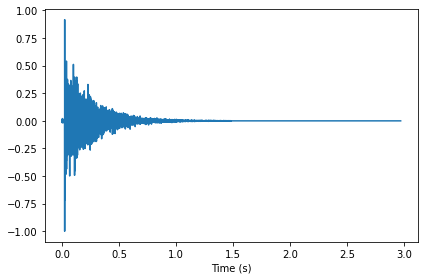
\includegraphics[width=0.6\linewidth]{resources/Images/task1_shot_wave}
        \caption{Полученный сигнал выстрела.}
        \label{fig:task1_shot_wave}
    \end{figure}

    Теперь посмотрим на его спектр.

    \begin{lstlisting}[caption= Получение спектра сигнала., label={lst:task1_shot_spectrum}]
transfer = shot.make_spectrum()
transfer.plot()
decorate(xlabel='Frequency (Hz)', ylabel='Amplitude')   \end{lstlisting}

    \begin{figure}[h]
        \centering
        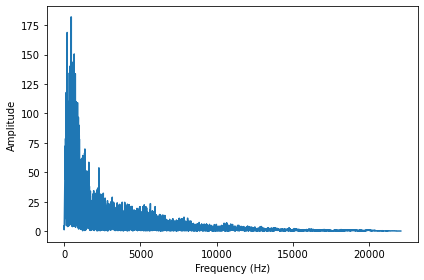
\includegraphics[width=0.8\linewidth]{resources/Images/task1_shot_spectrum}
        \caption{Спектр сигнала выстрела.}
        \label{fig:task1_shot_spectrum}
    \end{figure}

    \subsection{Скрипка}
    \label{subsec:task1_2}
    Теперь возьмём сигнал скрипки.

    \begin{lstlisting}[caption= Чтение и преобразование сигнала скрипки., label={lst:task1_violin_wave}]
violin = read_wave('resources/Sounds/task1_jcveliz_violin_origional.wav')
violin.make_audio()

violin = violin.segment(start=0.11)
violin.shift(-0.11)
violin.truncate(2**16)
violin.zero_pad(2**17)
violin.normalize()
violin.plot()
decorate(xlabel='Time (s)')     \end{lstlisting}

    Посмотрим на спектр полученного сигнала.

    \begin{lstlisting}[caption= Получение спектра сигнала скрипки., label={lst:task1_violin_spectrum}]
violin_spectrum = violin.make_spectrum()
violin_spectrum.plot()
decorate(xlabel='Frequency (Hz)', ylabel='Amplitude')       \end{lstlisting}

    \begin{figure}[H]
        \centering
        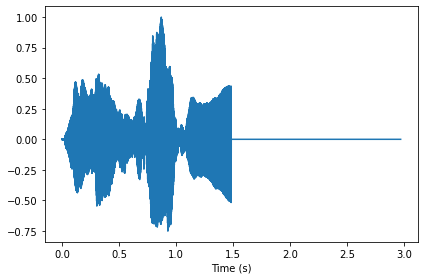
\includegraphics[width=0.7\linewidth]{resources/Images/task1_violin_wave}
        \caption{Полученный сигнал скрипки.}
        \label{fig:task1_violin_wave}
    \end{figure}

    \begin{figure}[H]
        \centering
        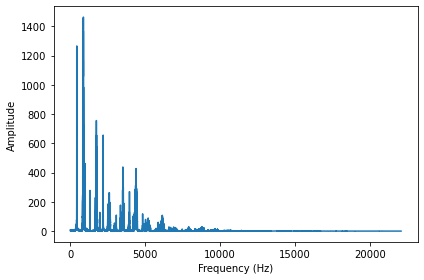
\includegraphics[width=0.7\linewidth]{resources/Images/task1_violin_spectrum}
        \caption{Спектр сигнала скрипки.}
        \label{fig:task1_violin_spectrum}
    \end{figure}

    Теперь умножим ДПФ сигнала на передаточную функцию и преобразуем полученный результат обратно в сигнал.

    \begin{lstlisting}[caption= Умножение ДПФ сигнала на передаточную функцию., label={lst:task1_violin_result}]
output = (violin_spectrum * transfer).make_wave()
output.normalize()
output.plot()
output.make_audio() \end{lstlisting}

    \begin{figure}[H]
        \centering
        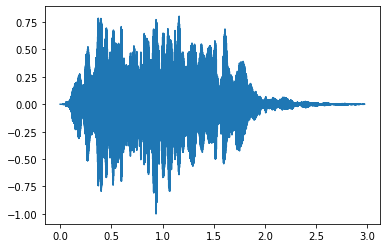
\includegraphics[width=0.8\linewidth]{resources/Images/task1_violin_result}
        \caption{Преобразованный сигнал скрипки.}
        \label{fig:task1_violin_result}
    \end{figure}

    При прослушивании полученного сигнала можно заметить, что лишней "затёкшей" ноты в начале нет.

    В данном упражнении был изучен способ устранения лишней ноты в начале фрагмента, возникающей в результате
    использования круговой свёртке. Это можно сделать, добавив достаточное количество нулей в конец сигнала, перед
    вычислением ДПФ.

    \newpage

% ---------------------------------------------- Упражнение 10.2 ----------------------------------------------
    \section{Упражнение 10.2}
    \label{sec:task2}

    В данном упражнении необходимо просмотреть коллекцию импульсных характеристик на онлайн-ресурсе
    \href{http://www.openairlib.net}{Open AIR} и скачать одну из них. Затем необходимо найти и скачать короткие записи
    с той же частотой дискретизации, что и у найденной импульсной характеристики. После этого необходимо смоделировать
    двумя способами звучание записи в том пространстве, где была измерена импульсная характеристика, как сверткой самой
    записи с импульсной характеристикой, так и умножением ДПФ записи на вычисленный фильтр, соответствующий импульсной
    характеристике.

    Итак, был выбрана \href{https://www.openair.hosted.york.ac.uk/?page_id=406}{эта} импульсная характеристика и
    \href{https://freesound.org/people/stomachache/sounds/231275/}{эта} запись звона колокольчиков.

    Теперь считаем импульсную характеристику. Это запись первой баптистской церкви в Нэшвилле.

    \begin{lstlisting}[caption= Чтение записи и формирование сигнала., label={lst:task2_response}]
response = read_wave('resources/Sounds/task2_1st_baptist_nashville_balcony.wav')
response = response.segment(duration=3)

response.normalize()
response.plot()
decorate(xlabel='Time (s)')
response.make_audio()   \end{lstlisting}

    \begin{figure}[h]
        \centering
        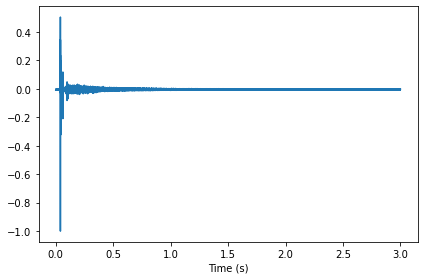
\includegraphics[width=0.7\linewidth]{resources/Images/task2_response}
        \caption{Сигнал импульсной характеристики.}
        \label{fig:task2_response}
    \end{figure}

    Теперь получим ДПФ импульсной характеристики - передаточную функцию.

    \begin{lstlisting}[caption= Получение передаточной функции., label={lst:task2_transfer}]
transfer = response.make_spectrum()
transfer.plot()
decorate(xlabel='Frequency (Hz)', ylabel='Amplitude')   \end{lstlisting}

    \begin{figure}[H]
        \centering
        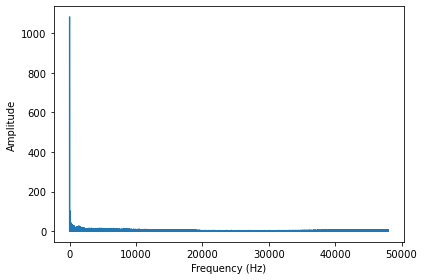
\includegraphics[width=0.7\linewidth]{resources/Images/task2_transfer}
        \caption{Передаточная функция.}
        \label{fig:task2_transfer}
    \end{figure}

    Посмотрим на неё в логарифмическом масштабе.

    \begin{lstlisting}[caption= Преобразование передаточной функции в логарифмичский масштаб., label={lst:task2_transfer_log}]
transfer.plot()
decorate(xlabel='Frequency (Hz)', ylabel='Amplitude', xscale='log', yscale='log')   \end{lstlisting}

    \begin{figure}[H]
        \centering
        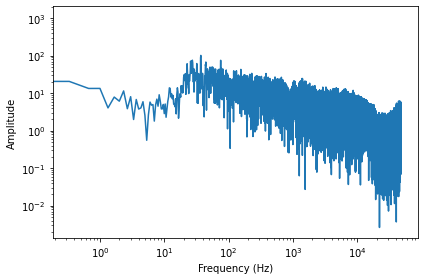
\includegraphics[width=0.7\linewidth]{resources/Images/task2_transfer_log}
        \caption{Передаточная функция в логарифмическом масштабе.}
        \label{fig:task2_transfer_log}
    \end{figure}

    Теперь считаем запись колокольчиков.

    \begin{lstlisting}[caption= Чтение записи колокольчиков., label={lst:task2_bell_wave}]
bell_wave = read_wave('resources/Sounds/task2_stomachache_cowbell.wav')
bell_wave = bell_wave.segment(start=0)

bell_wave.truncate(len(response))
bell_wave.normalize()
bell_wave.plot()
decorate(xlabel='Time (s)')
bell_wave.make_audio()      \end{lstlisting}

    \begin{figure}[h]
        \centering
        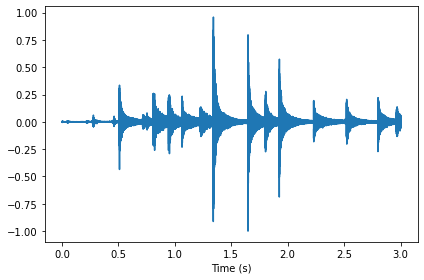
\includegraphics[width=0.8\linewidth]{resources/Images/task2_bell_wave}
        \caption{Сигнал колокольчиков.}
        \label{fig:task2_bell_wave}
    \end{figure}

    Вычислим ДПФ записи колокольчиков.

    \begin{lstlisting}[caption= Получение ДПФ записи колокольчиков., label={lst:task2_bell_spectrum}]
bell_spectrum = bell_wave.make_spectrum()
bell_spectrum.plot()
decorate(xlabel='Frequency (Hz)', ylabel='Amplitude')   \end{lstlisting}

    Теперь смоделируем звучание колокольчиков в пространстве, умножив ДПФ нашей записи на вычисленный фильтр импульсной
    характеристики.

    \begin{lstlisting}[caption= Умножение ДПФ записи на фильтр., label={lst:task2_bell_result}]
output = (bell_spectrum * transfer).make_wave()
output.normalize()
output.plot()
output.make_audio()     \end{lstlisting}

    \begin{figure}[H]
        \centering
        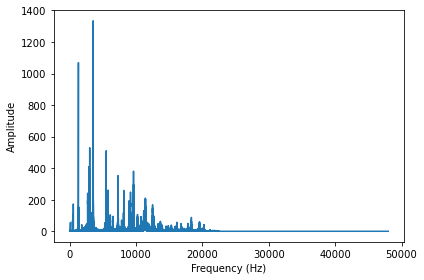
\includegraphics[width=0.8\linewidth]{resources/Images/task2_bell_spectrum}
        \caption{ДПФ записи колокольчиков.}
        \label{fig:task2_bell_spectrum}
    \end{figure}

    \begin{figure}[H]
        \centering
        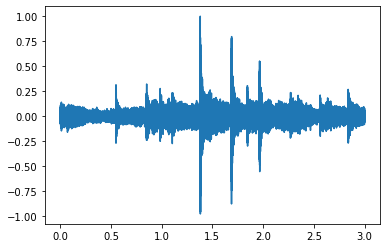
\includegraphics[width=0.8\linewidth]{resources/Images/task2_bell_result}
        \caption{Смоделированный сигнал.}
        \label{fig:task2_bell_result}
    \end{figure}

    Прослушав полученный сигнал, можно заметить, что звук действительно как будто переместился в большое пространство,
    появились эхо и небольшой гул на фоне.

    Теперь используем свертку.

    \begin{lstlisting}[caption= Использование свертки., label={lst:task2_bell_convolve}]
convolved2 = bell_wave.convolve(response)
convolved2.normalize()
convolved2.make_audio()
    \end{lstlisting}

    Сигнал, полученный таким образом, звучит так же, как и предыдущий.

    В данном упражнении было смоделировано звучание записи колокольчиков в выбранном пространстве, где была измерена
    импульсная характеристика, двумя способами: умножением ДПФ на вычисленный фильтр и сверткой.
    При сравнении полученных записей был сделан вывод, что полученные записи звучат одинаково.
    \newpage

% ---------------------------------------------- Выводы ----------------------------------------------
    \section{Выводы}
    \label{sec:conclusions}

    В ходе выполнения данной лабораторной работы был изучен вариант решения проблемы возникновения "затекшей" ноты в
    начале фрагмента при использовании свертки. Был сделан вывод, что дополнение нулями устраняет эту лишнюю ноту.

    Кроме того, было смоделировано звучание записи колокольчиков в выбранном пространстве двумя способами:
    умножением ДПФ на вычисленный фильтр и сверткой. Был сделан вывод, что записи, полученные этими способами, звучат
    одинаково.
\end{document}